\chapter{Ansible, Puppet, and Chef}\label{ansible-puppet-and-chef}

\section{Configuration Drift}\label{configuration-drift}

\begin{itemize}
\tightlist
\item
  CONFIGURATION DRIFT is when individual changes made over time causes a
  device's configuration to deviate from the standard / correct
  configurations as defined by the company

  \begin{itemize}
  \tightlist
  \item
    Although each device will have unique parts of its configurations
    (IP Addresses, hostname, etc) most of a device's configuration is
    usually defined in standard templates designed by the network
    architects / engineers of the company
  \item
    As individual engineers make changes to devices (for example, to
    troubleshoot and fix network issues, test configurations, etc), the
    configuration of a device can drift away from the standard.
  \item
    Records of these individual changes and their reasons aren't kept
  \item
    This can lead to future issues
  \end{itemize}
\item
  Even without automation tools, it is best to have standard
  configuration management practices.

  \begin{itemize}
  \tightlist
  \item
    When a change is made, save the config as a text file and place it
    in a shared folder

    \begin{itemize}
    \tightlist
    \item
      A standard naming system like (\emph{hostname\_yyyymmdd)} might be
      used.
    \item
      There are flaws to this system, as an engineer might forget to
      place the new config in the folder after making changes. Which one
      should be considered the ``CORRECT'' config?
    \item
      Even if configurations are properly saved like this, it doesn't
      guarantee that the configurations actually match the standard
    \end{itemize}
  \end{itemize}
\end{itemize}

\section{Configuration Provisioning}\label{configuration-provisioning}

\begin{itemize}
\item
  CONFIGURATION PROVISIONING refers to how configuration changes are
  applied to devices

  \begin{itemize}
  \tightlist
  \item
    This includes configuring new devices, too
  \end{itemize}
\item
  Traditionally, configuration provisioning is done by connecting to
  devices one-by-one via SSH

  \begin{itemize}
  \tightlist
  \item
    This is not practical in large networks
  \end{itemize}
\item
  Configuration management tools like Ansible, Puppet, and Chef allow us
  to make changes to devices on a mass scale with a fraction of time and
  effort.
\item
  TWO ESSENTIAL COMPONENTS:

  \begin{itemize}
  \tightlist
  \item
    Templates
  \item
    Variables
  \end{itemize}
\end{itemize}

\begin{figure}
\centering
\pandocbounded{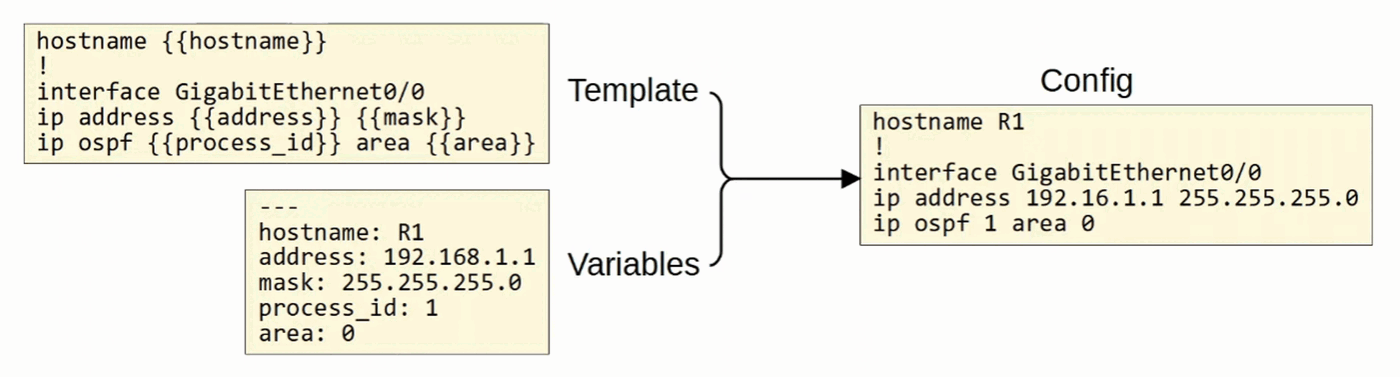
\includegraphics[keepaspectratio,alt={image}]{images/66-ansible-puppet-chef/img-001.png}}
\end{figure}

\section{Intro to Configuration Management
Tools}\label{intro-to-configuration-management-tools}

\begin{itemize}
\tightlist
\item
  CONFIGURATION MANAGEMENT TOOLS are network automation tools that
  facilitate the centralized control of large numbers of network devices
\item
  The option you need to be aware of for the CCNA are Ansible, Puppet,
  and Chef
\item
  These tools were originally developed after the rise of VMs, to enable
  server system admins to automate the process of creating, configuring,
  and removing VMs

  \begin{itemize}
  \tightlist
  \item
    However, they are also widely used to manage network devices
  \end{itemize}
\item
  These tools can be used to perform tasks such as :

  \begin{itemize}
  \tightlist
  \item
    Generate configurations for new devices on a large scale
  \item
    Perform configuration changes on devices (all devices in your
    network, or certain subset of devices)
  \item
    Check device configurations for compliance with defined standards
  \item
    Compare configurations between devices, and between different
    versions of configurations on the same device
  \end{itemize}
\end{itemize}

\begin{figure}
\centering
\pandocbounded{
\includegraphics[keepaspectratio,alt={image}]{images/66-ansible-puppet-chef/img-002.png}}
\end{figure}

\section{Ansible}\label{ansible}

\begin{itemize}
\tightlist
\item
  ANSIBLE is a configuration management tool owned by Red Hat
\item
  Ansible itself is written in Python
\item
  Ansible is \emph{agentless}

  \begin{itemize}
  \tightlist
  \item
    It doesn't require any special software to run on the managed
    devices
  \end{itemize}
\item
  Ansible uses SSH to connect to devices, make configuration changes,
  extract info, etc
\item
  Ansible uses a \emph{push} model. The Ansible server (Control node)
  uses SSH to connect to managed devices and \emph{push} configuration
  changes to them

  \begin{itemize}
  \tightlist
  \item
    Puppet and Chef use a \emph{pull} model
  \end{itemize}
\item
  After installing Ansible itself, you must create several text files:

  \begin{itemize}
  \tightlist
  \item
    PLAYBOOKS :

    \begin{itemize}
    \tightlist
    \item
      These files are ``blueprints of automation tasks''
    \item
      They outline the logic and actions of the tasks that Ansible
      should do
    \item
      Written in YAML
    \end{itemize}
  \item
    INVENTORY :

    \begin{itemize}
    \tightlist
    \item
      These files list the devices that will be managed by Ansible, as
      well as characteristics of each device such as their device role
      (Access Switch, Core Switch, WAN Router, Firewall, etc.)
    \item
      Written in INI, YAML, or other formats
    \end{itemize}
  \item
    TEMPLATES :

    \begin{itemize}
    \tightlist
    \item
      These files represent a device's configuration file, but specific
      values for variables are not provided.
    \item
      Written in JINJA2 format
    \end{itemize}
  \item
    VARIABLES :

    \begin{itemize}
    \tightlist
    \item
      These files list variables and their values.
    \item
      These values are substituted into the templates to create complete
      configuration files.
    \item
      Written in YAML
    \end{itemize}
  \end{itemize}
\end{itemize}

\begin{figure}
\centering
\pandocbounded{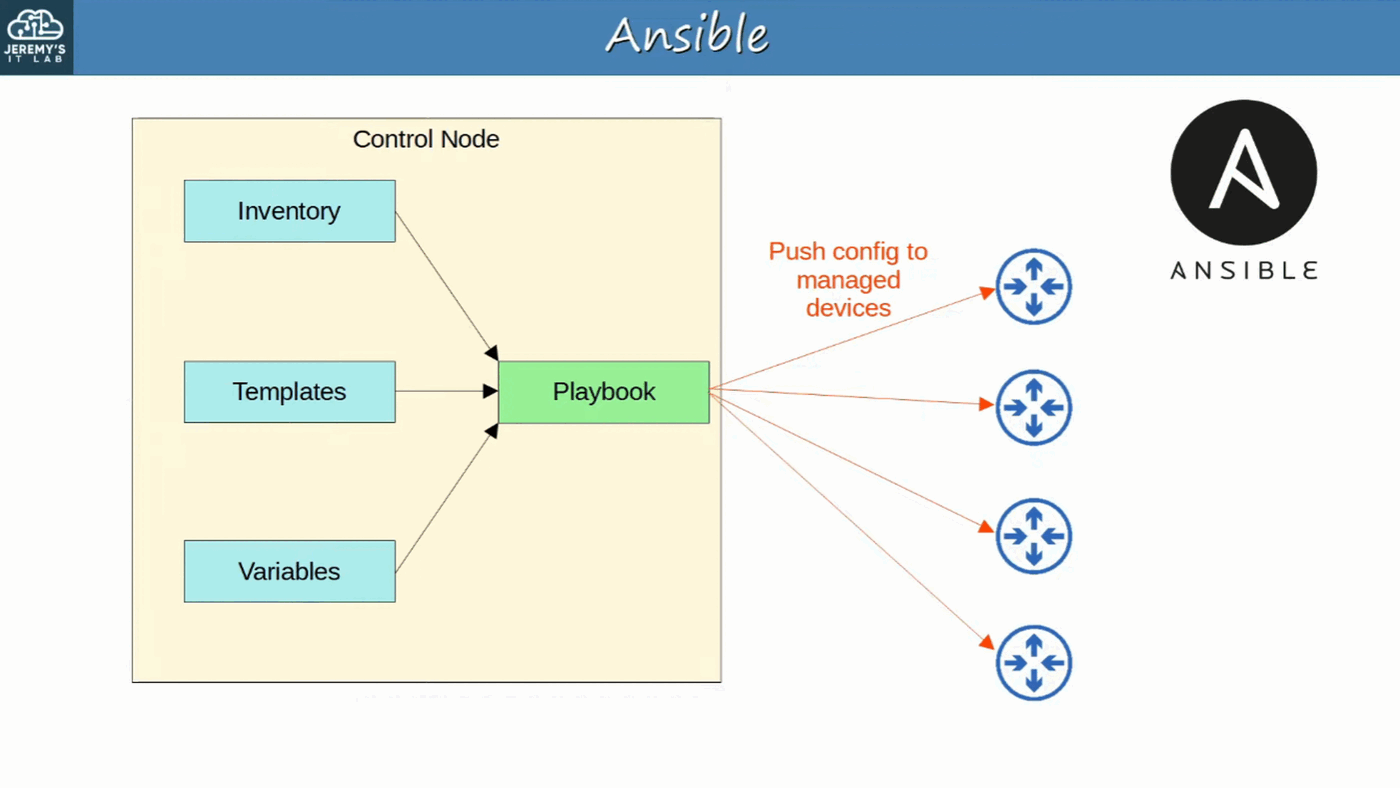
\includegraphics[keepaspectratio,alt={image}]{images/66-ansible-puppet-chef/img-003.png}}
\end{figure}

\section{Puppet}\label{puppet}

\begin{itemize}
\tightlist
\item
  PUPPET is a configuration management tool written in RUBY
\item
  Puppet is typically agent-based

  \begin{itemize}
  \tightlist
  \item
    Specific software must be installed on the managed devices
  \item
    Not all Cisco devices support a Puppet agent
  \end{itemize}
\item
  It CAN be run \emph{agentless,} in which a proxy agent runs on an
  external host, and a proxy agent uses SSH to connect to the managed
  devices and communicate with them
\item
  The Puppet server is called the ``Puppet master''
\item
  Puppet uses a PULL model (clients ``pull'' configurations from the
  Puppet master)

  \begin{itemize}
  \tightlist
  \item
    Clients use TCP 8140 to communicate with the Puppet master
  \end{itemize}
\item
  Instead of YAML, it uses a proprietary language for files
\item
  Text files required on the Puppet master include:

  \begin{itemize}
  \tightlist
  \item
    MANIFEST :

    \begin{itemize}
    \tightlist
    \item
      The file defines the desired configuration state of a network
      device
    \end{itemize}
  \item
    TEMPLATES :

    \begin{itemize}
    \tightlist
    \item
      Similar to Ansible templates.
    \item
      Used to generate MANIFESTS
    \end{itemize}
  \end{itemize}
\end{itemize}

\begin{figure}
\centering
\pandocbounded{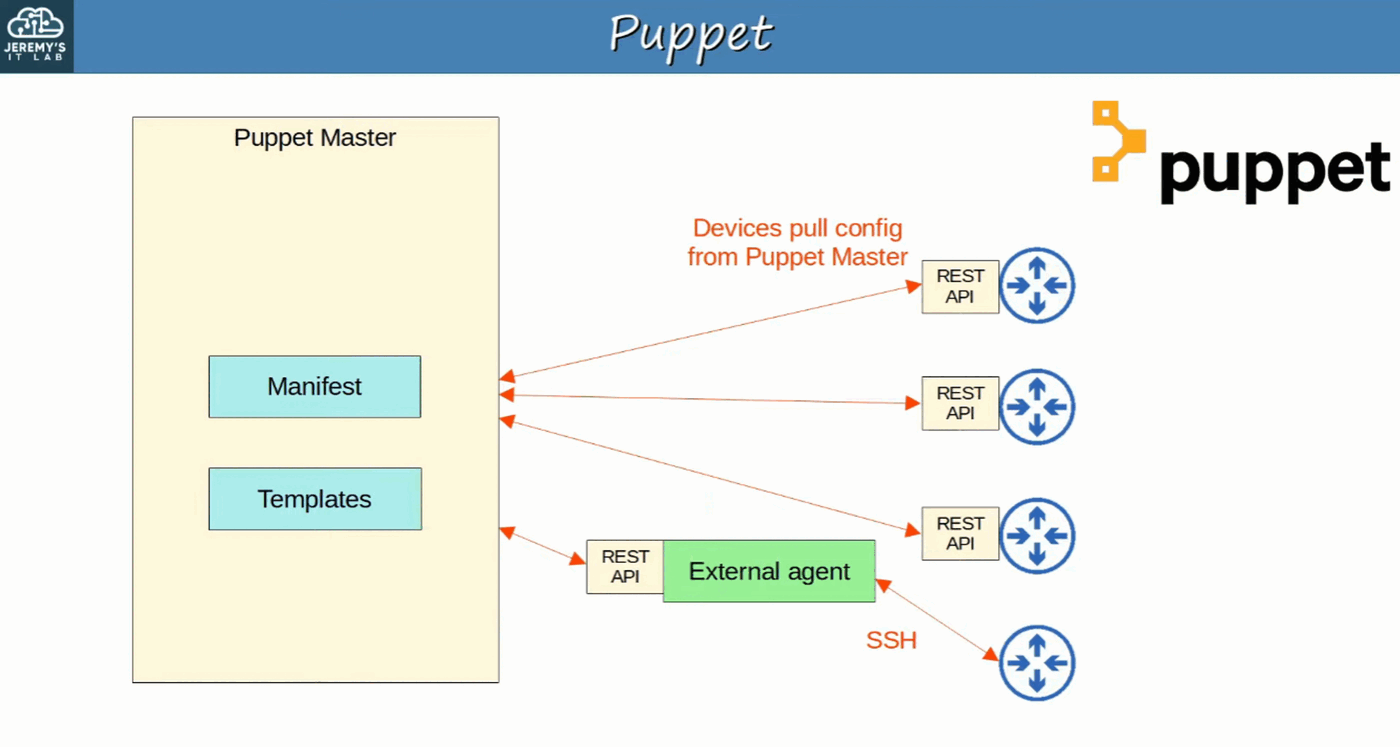
\includegraphics[keepaspectratio,alt={image}]{images/66-ansible-puppet-chef/img-004.png}}
\end{figure}

\section{Chef}\label{chef}

\begin{itemize}
\tightlist
\item
  CHEF is a configuration management tool written in RUBY
\item
  CHEF is Agent-Based

  \begin{itemize}
  \tightlist
  \item
    Specific software must be installed on the managed devices
  \item
    Not all Cisco devices support a CHEF agent
  \end{itemize}
\item
  CHEF uses a PULL model
\item
  The server uses TCP 10002 to send configurations to clients
\item
  Files use a DSL (Domain-Specific Language) based on Ruby
\item
  Text files used by CHEF include:

  \begin{itemize}
  \tightlist
  \item
    RESOURCES :

    \begin{itemize}
    \tightlist
    \item
      The ``ingredients'' in a RECIPE.
    \item
      Configuration objects managed by CHEF
    \end{itemize}
  \item
    RECIPES :

    \begin{itemize}
    \tightlist
    \item
      The ``recipes'' in a COOKBOOK.
    \item
      Outlines the logic and actions of the tasks performed on the
      resources
    \end{itemize}
  \item
    COOKBOOKS :

    \begin{itemize}
    \tightlist
    \item
      A set of related RECIPES grouped together
    \end{itemize}
  \item
    RUN-LIST :

    \begin{itemize}
    \tightlist
    \item
      An ordered list of RECIPES that are run to bring a device to the
      desired configuration state
    \end{itemize}
  \end{itemize}
\end{itemize}

\begin{figure}
\centering
\pandocbounded{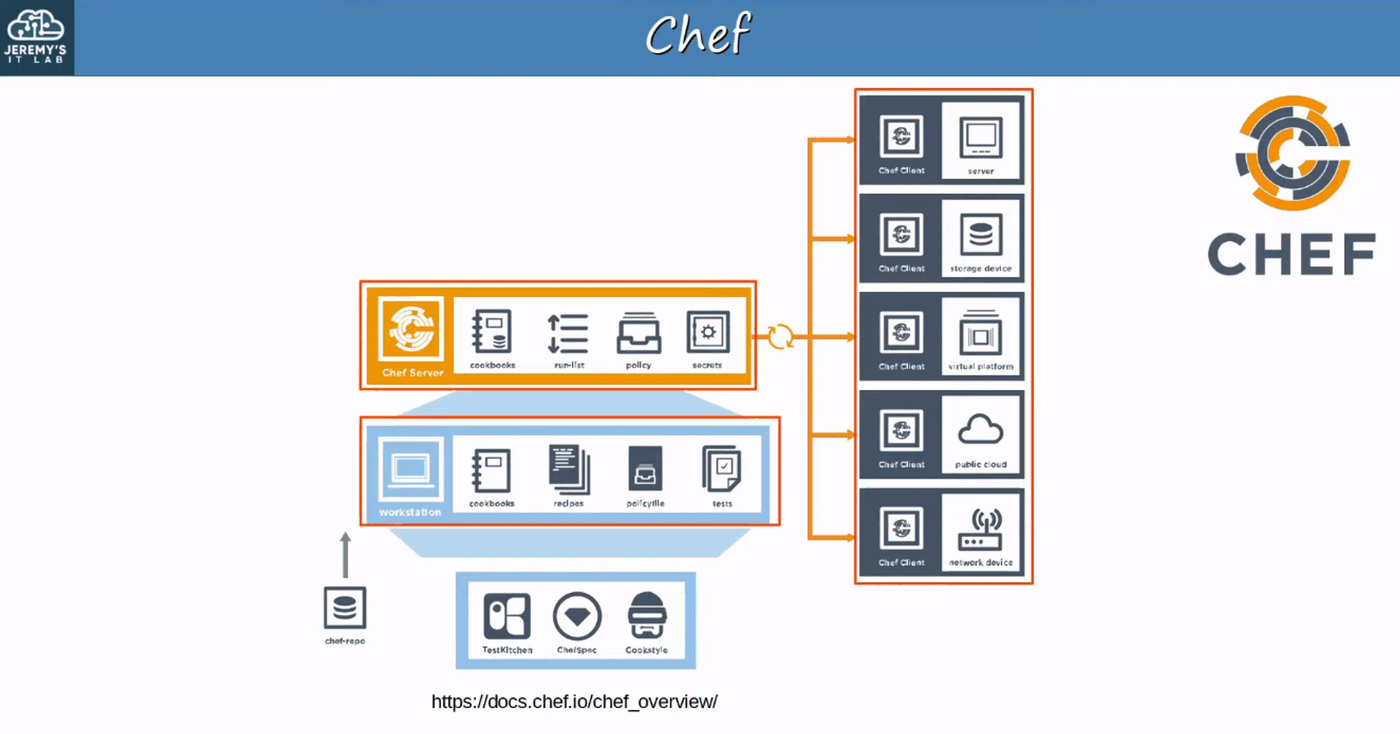
\includegraphics[keepaspectratio,alt={image}]{images/66-ansible-puppet-chef/img-005.png}}
\end{figure}

\section{Memorize This Chart for the
CCNA}\label{memorize-this-chart-for-the-ccna}

\begin{figure}
\centering
\pandocbounded{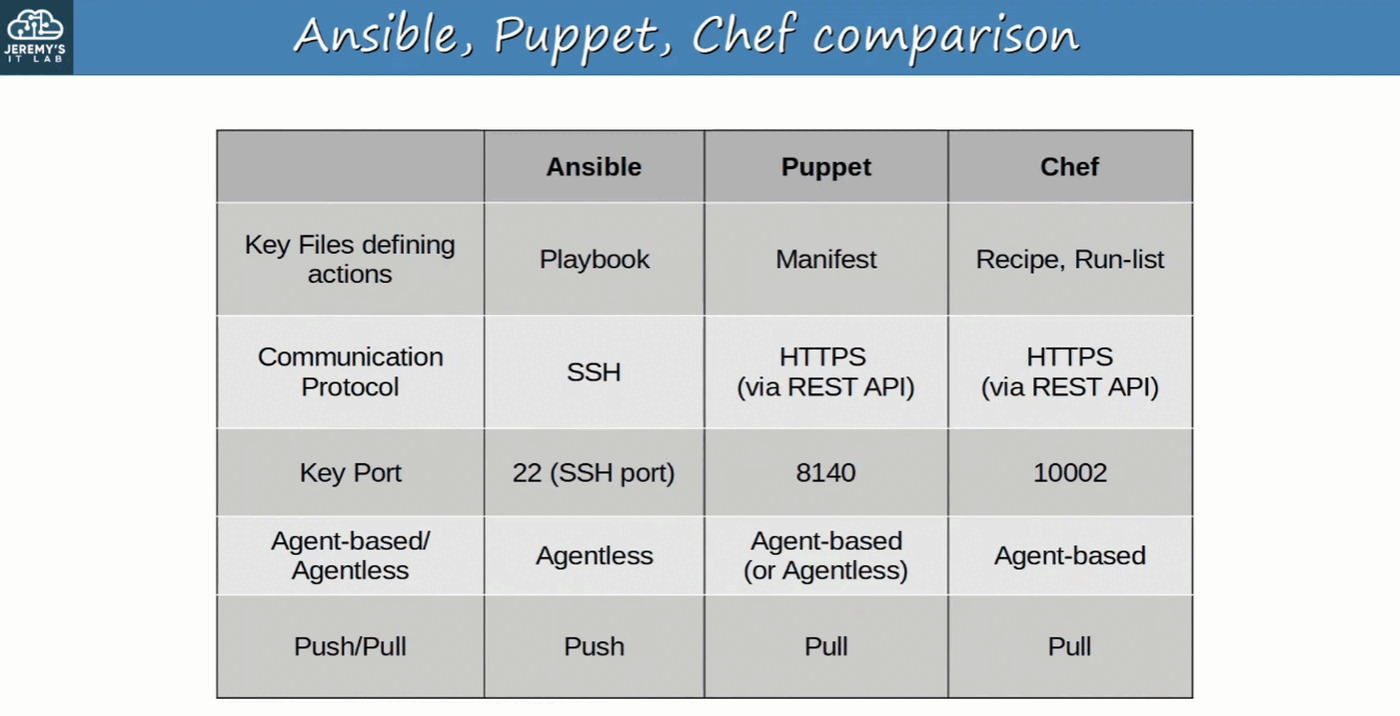
\includegraphics[keepaspectratio,alt={image}]{images/66-ansible-puppet-chef/img-006.png}}
\end{figure}
